\section{Experiments}
\label{sec:experiments}

\subsection{The influence of label noises in segmention}
\label{subsec:robustness}

%%%%%%%% TEXT Experiment setup

To investigate the influence of the lablel noises, (1) inexhaustive segmentations, (2) objects mislabelling and (3) false positive segmentations, on the learned representations, we set up experiments with simulated label noises from a well-annotated dataset, the PASCAL VOC2011 segmentation dataset \cite{everingham2015pascal}.

\paragraph{Dataset}
In this experiment, fifteen out of twenty categories of the VOC2011 dataset were selected to form a \textit{pre-training dataset} and the other categories formed a \textit{fine-tuning dataset}.
The pre-training dataset was used to train a Fully Convolutional Network with AlexNet (FCN-AlexNet) model \cite{long2015fully} for segmentation in the presence or absence of simulated label noises.
Inexhaustive segmentations, objects mislabelling, and false segmentations were simulated independently with stochastical corruptions to the well-annotated pre-training dataset, followed the descriptions in Section \ref{subsec:formulation}.
The fine-tuning dataset was used to fine-tune the weights of convolutional layers from the pre-trained FCN-AlexNet models.
To avoid that the choice of pre-training and fine-tuning splitting for categories influence the results, the 20 categories of VOC2011 were divided equally into four folds.
The training dataset was enriched with extra segmentations by Hariharan et al. \cite{hariharan2011semantic}
To keep the segmentation task simple, we used only single-object images, resulting in totally 4000 training images for 20 categories available for pre-training, fine-tuning and evaluation.
We subsampled the original images by four times to accelerate the training process.

\paragraph{Experimental setup}
The fine-tuned models were evaluated by mean intersection over union ratio (mean IU) achieved on the fine-tuning test set, referring to as the \textit{fine-tuning performance}.
Performance improvement of fine-tuning transferred models compared to a randomly initialized model indicates the transferability of pre-trained weights.
The non-transferable layers of FCN-AlexNet were randomly initialized with Xavier Initialization.
Experiments run for each fold independently, and the exact partitions of each fold are listed in Table \ref{tab:robustness}.
Fully Convolutional Networks with AlexNet was used for experiments because of its relatively small capacity and thus short training time.
The pre-trained AlexNet model was used to set a baseline of performance, denoted as the ImageNet model.
The ImageNet model and completely random weight initialization were considered as the upper baseline and lower baseline, respectively, for various pre-trained weights summarized in Table \ref{tab:robustness}.
The default hyperparameters of FCN-AlexNet in  \cite{long2015fully} were kept unchanged.
The training process run 240,000 iterations for pre-training phase, and 12,000 iterations for fine-tuning phase.
Snapshots for trained models were taken every 4,000 iterations.
Each experiment was repeated three times, mean and standard deviation were computed over the last five snapshots for all repetitions.


% \noindent \textit{What Table \ref{tab:robustness} tell us.
% How annotation errors were synthesized;
% How synthesizations are different from reality;
% Transferability of noisy models compared to clean models.
% }

\paragraph{Objects mislabelling}
The negative influence of random object labels on feature transferability is demonstrated in Table \ref{tab:robustness}.
Compared to the model trained with true labels, both models trained with all random labels and half true half random labels are less transferable to the fine-tuning dataset.
Transferring the AllRandomLabels model or the HalfRandomLabels model is no better than randomly initializing model weights.
The mislabeled objects in segmentations negatively impact the transferability of CNN models in this simulated experiment setup.

We then binarize pre-training classes to foreground and background and achieve a fine-tuning performance better than training with the exact (half) randomized labels and equivalent to training with correct labels.
Randomized object labels were mislabeled among foreground classes so that binarizing labels a foreground and background classes can in a sense correct the randomized labels.
Compared to the precise but inaccurate noisy labels, binarized labels are accurate but imprecise.
This observation indicates that inaccurate labels have a larger influence on the learned representations than imprecise labels.


\paragraph{Precise labels vs. Accurate labels}
To validate that accurate, imprecise labels have less negative effect on feature transferability than inaccurate, precise labels.
In figure \ref{fig:categories}, we decrease the preciseness of pre-training labels by grouping the pre-training classes into a various number of categories to demonstrate the corresponding change of feature transferability.
Addition to the binary categorization, we also categorized the fifteen pre-training classes into four meaningful categories: person, animal, vehicle, indoor according to \cite{everingham2015pascal}.
The result transferred and fine-tuned model is shown as the error bars on the solid line at categories=4.
It has almost the same fine-tuning performance as the model trained with binarized labels and the model trained with precision labels (shown as error bar at categories=15).

As a comparison, the fifteen classes were randomly categorized into 4, 7, 11 categories and shown as isolated error bars in figure \ref{fig:categories} at categories=4, 7, 11 respectively.
Figure \ref{fig:categories} reveals that reducing label preciseness by categorizing pre-training classes has little effect on the fine-tuning performance of transferred models.
Even categorizing classes at random without explicit meaning can pre-train weights better than random initialization (shown as error bar at categories=0).

In contrast to the significant influence of randomized precise labels, the imprecise binarized labels have little effect to the learned representations.
Binarizing is helpful to learn better representations when mislabeled objects is dominant.

\paragraph{Inexaustive segmentation}
Fine-tuning performance for pre-trained models with complete segmentations and incomplete segmentations are summarized in Table \ref{tab:robustness}.
Pre-training data with half of the objects unsegmented results in fine-tuned models with a worse mean IU (average across four folds) than pre-training with complete labels by 0.04, the same as no pre-training.
This observation demonstrates that inexhaustive segmentations have a negative impact on representations transferability.
% In a positive and unlabeled (PU) learning setting, not only the classification performance but also the transferability of learned weights decreases due to the noises in negative labels.

By applying the class-dependent sigmoid loss to pre-train models with half of the objects segmented, a fine-tuning performance comparable to the model pre-trained with complete segmentation is achieved.
The class-dependent sigmoid loss compensates the negative influence of inexhaustive segmentations on the fine-tuning performance of the pre-trained model.
% The negative influence of inexhaustive segmentations on the fine-tuning performance of the pre-traine model is compensated.
Note that we train foreground/background segmentation instead of multi-class segmentation when applied the class-dependent sigmoid loss because binary segmentation can produce as good representation as multi-class segmentation.
% The details of implementing sigmoid negative loss for the pre-training dataset will be discussed in Section \ref{subsec:pulearning}.


\paragraph{False positive segmentations}
We observe a little influence of the incorrectly segmented objects from the non-predefined but meaningful categories, i.e., the false positive segmentations, on the learned representations.
To simulate the false positive segmentations errors, we selected one category, either cat or dog depending on the folds, as the target category and all the other 14 categories in the pre-training dataset became non-target, as discussed in Section \ref{subsec:formulation}.
In the presence of false segmentations, instances from non-target categories can be misannotated as the target category with a probability of $p_{10}= 0.5$.
The result pre-trained models is named as the HalfFalsePositive model in Table \ref{tab:robustness}.
The noise-free counterpart of is the model pre-trained with segmentations of the selected target category only, and the other 14 categories remained unsegmented, denoted as the NoFalsePositive model.

We observe from Table \ref{tab:robustness} that transferring the HalfFalsePositive model performs almost the same as the NoFalsePositive model.
Therefore, false positive segmentation for objects from the 14 categories have a little negative impact on pre-training CNN models.
% The exact influence of false segmentations in practice, however, may depend on how similar the target and non-target categories are, or whether false segmentations are consistent, which requires further investigation.

\begin{table*}[t]
\resizebox{\textwidth}{!}{
\centering
\begin{tabular}{l|l|llll|l}

\hline
                                                                                      & \begin{tabular}[c]{@{}c@{}}Initial Feature\\ Extractor\end{tabular} & \multicolumn{4}{c|}{Fine-tuning mean IU per pretraining-finetuning fold}                                                                                                                                                                                                                                                                                                                                                                     & \multicolumn{1}{l}{\multirow{2}{*}{\begin{tabular}[c]{@{}l@{}}Average \\ mean IU\\ across \\ four folds\end{tabular}}} \\ \cline{1-6}
\begin{tabular}[c]{@{}l@{}}Fine-tuning\\ categories\end{tabular}                      &                                                                     & \multicolumn{1}{l}{\begin{tabular}[c]{@{}l@{}}aeroplane, \\ bicycle, bird,\\ boat, bottle\end{tabular}} & \multicolumn{1}{l}{\begin{tabular}[c]{@{}l@{}}bus, car, \\ cat, \\ chair, cow\end{tabular}} & \multicolumn{1}{l}{\begin{tabular}[c]{@{}l@{}}dining table,\\ dog, horse, \\ motorbike,\\ person\end{tabular}} & \multicolumn{1}{l|}{\begin{tabular}[c]{@{}l@{}}potted plant, \\ sheep, sofa, \\ train, TV\end{tabular}} & \multicolumn{1}{l}{}                                                                                                   \\ \hline
\multirow{2}{*}{\begin{tabular}[c]{@{}l@{}}Baseline\end{tabular}} & ImageNetModel                                                       & $0.42\pm0.01$                                                                                           & $0.51\pm0.01$                                                                               & $0.49\pm0.01$                                                                                                  & $0.47\pm0.01$                                                                                           & $0.47\pm0.01$                                                                                                          \\
                                                                                      & RandomWeights                                                       & $0.29\pm0.01$                                                                                           & $0.29\pm0.03$                                                                               & $0.27\pm0.01$                                                                                                  & $0.30\pm0.02$                                                                                           & $0.29\pm0.02$                                                                                                          \\ \hline
\multirow{4}{*}{\begin{tabular}[c]{@{}l@{}}Objects \\ Mislabelling\end{tabular}}       & TrueLabels                                                      & $0.29\pm0.01$                                                                                           & $0.36\pm0.01$                                                                               & $0.29\pm0.01$                                                                                                  & $0.37\pm0.01$                                                                                           & $\mathbf{0.33\pm0.01}$                                                                                                 \\
                                                                                      & AllRandomLabels                                                     & $0.29\pm0.01$                                                                                           & $0.33\pm0.03$                                                                               & $0.26\pm0.01$                                                                                                  & $0.28\pm0.01$                                                                                           & $0.29\pm0.01$                                                                                                          \\
                                                                                      & HalfRandomLabels                                                    & $0.27\pm0.01$                                                                                           & $0.33\pm0.02$                                                                               & $0.25\pm0.01$                                                                                                  & $0.29\pm0.01$                                                                                           & $0.29\pm0.01$                                                                                                          \\
                                                                                      & BinarizedLabels                                                     & $0.30\pm0.02$                                                                                           & $0.35\pm0.01$                                                                               & $0.29\pm0.02$                                                                                                  & $0.35\pm0.03$                                                                                           & $\mathbf{0.32\pm0.02}$                                                                                                 \\ \hline
\multirow{3}{*}{\begin{tabular}[c]{@{}l@{}}Inexaustive \\ segmention\end{tabular}}    & CompleteLabels                                                      & $0.29\pm0.01$                                                                                           & $0.36\pm0.01$                                                                               & $0.29\pm0.01$                                                                                                  & $0.37\pm0.01$                                                                                           & $\mathbf{0.33\pm0.01}$                                                                                                 \\
                                                                                      & HalfUnsegmented                                                     & $0.26\pm0.01$                                                                                           & $0.30\pm0.03$                                                                               & $0.28\pm0.03$                                                                                                  & $0.32\pm0.02$                                                                                           & $0.29\pm0.02$                                                                                                          \\
                                                                                      & SigmoidLoss                                                       & \multicolumn{1}{l}{$0.30\pm0.01$}                                                                       & \multicolumn{1}{l}{$0.37\pm0.01$}                                                           & \multicolumn{1}{l}{$0.31\pm0.02$}                                                                              & \multicolumn{1}{l|}{$0.34\pm0.02$}                                                                      & $\mathbf{0.33\pm0.02}$                                                                                                 \\ \hline
\multirow{2}{*}{\begin{tabular}[c]{@{}l@{}}False positive \\ segmentaion\end{tabular}}         & NoFalsePositive                                                    & $0.26\pm0.01$                                                                                           & $0.37\pm0.03$                                                                               & $0.27\pm0.01$                                                                                                  & $0.33\pm0.04$                                                                                           & $\mathbf{0.31\pm0.02}$                                                                                                 \\
                                                                                      & HalfFalsePositive                                                  & \multicolumn{1}{l}{$0.27\pm0.01$}                                                                       & \multicolumn{1}{l}{$0.34\pm0.01$}                                                           & \multicolumn{1}{l}{$0.30\pm0.01$}                                                                              & \multicolumn{1}{l|}{$0.32\pm0.01$}                                                                      & $\mathbf{0.31\pm0.01}$                                                                                                 \\ \hline

\end{tabular}
}
\caption{
Segmentation performance for fine-tuned FCN-AlexNet models pre-trained on 15 categories from the PASCAL VOC2011 dataset and fine-tuned on the other 5 categories.
\textbf{ImageNetModel} represents the pre-trained ImageNet model;
\textbf{RandomWeights} indicates that the randomly initialized weights;
All the other extractors were pre-trained in the presence/absence of the corresponding label noises listed in the leftmost column.
Half of the objects unsegmented (\textbf{HalfUnsegmented}) result in pre-trained models not better than random weight initialization.
Introducing the sigmoid negative loss in the pre-training phase was able to improve the fine-tuning performance to be comparable to pre-trained model with complete segmentation (\textbf{CompleteLabels}).
Using random labels (\textbf{RamdomLabels}) decreased the fine-tuning performance of transferred models, compared to using true labels (\textbf{TrueLabels}).
Binarizing the pre-training classes as foreground and background help overcome the negative effects of random labels.
Applying the sigmoid loss to the negative class when pre-trained with inexhaustive segmentations achieves a comparable fine-tuning performance to pre-training with the complete segmentations.
Including the false positive segmentations in pre-training (\textbf{HalfFalsePositive}) achieves the same fine-tuning performance as not including the false positive segmentations (\textbf{NoFalsePositive}), better than random initialization.
% \textit{SingleCategory} was pre-trained on only one annotated category, either ``dog'' or ``cat'' depending on the fold, and the other categories were left unannotated;
% \textit{BinaryLabels} was pre-trained with binary labels that any objects of the fifteen categories were annotated as one single category, namely ``dog'' or ``cat'' depending on fold;
% \textit{TrueLabels} was pre-trained with all objects segmented and assigned to 15 categories correctly;
% \textit{AllRandomLabels} was pre-trained with all objects correctly segmented but assigned random labels;
% \textit{HalfRandomLabels} was pre-trained with all objects correctly segmented and half of them randomly assigned labels;
% \textit{IncompleteLabels} was trained with datasets that objects were annotated correctly with a probability of 0.5;
}
\label{tab:robustness}
\end{table*}


%%%%%%%% Figure categorizing classes
\begin{figure}[t]
\centering
   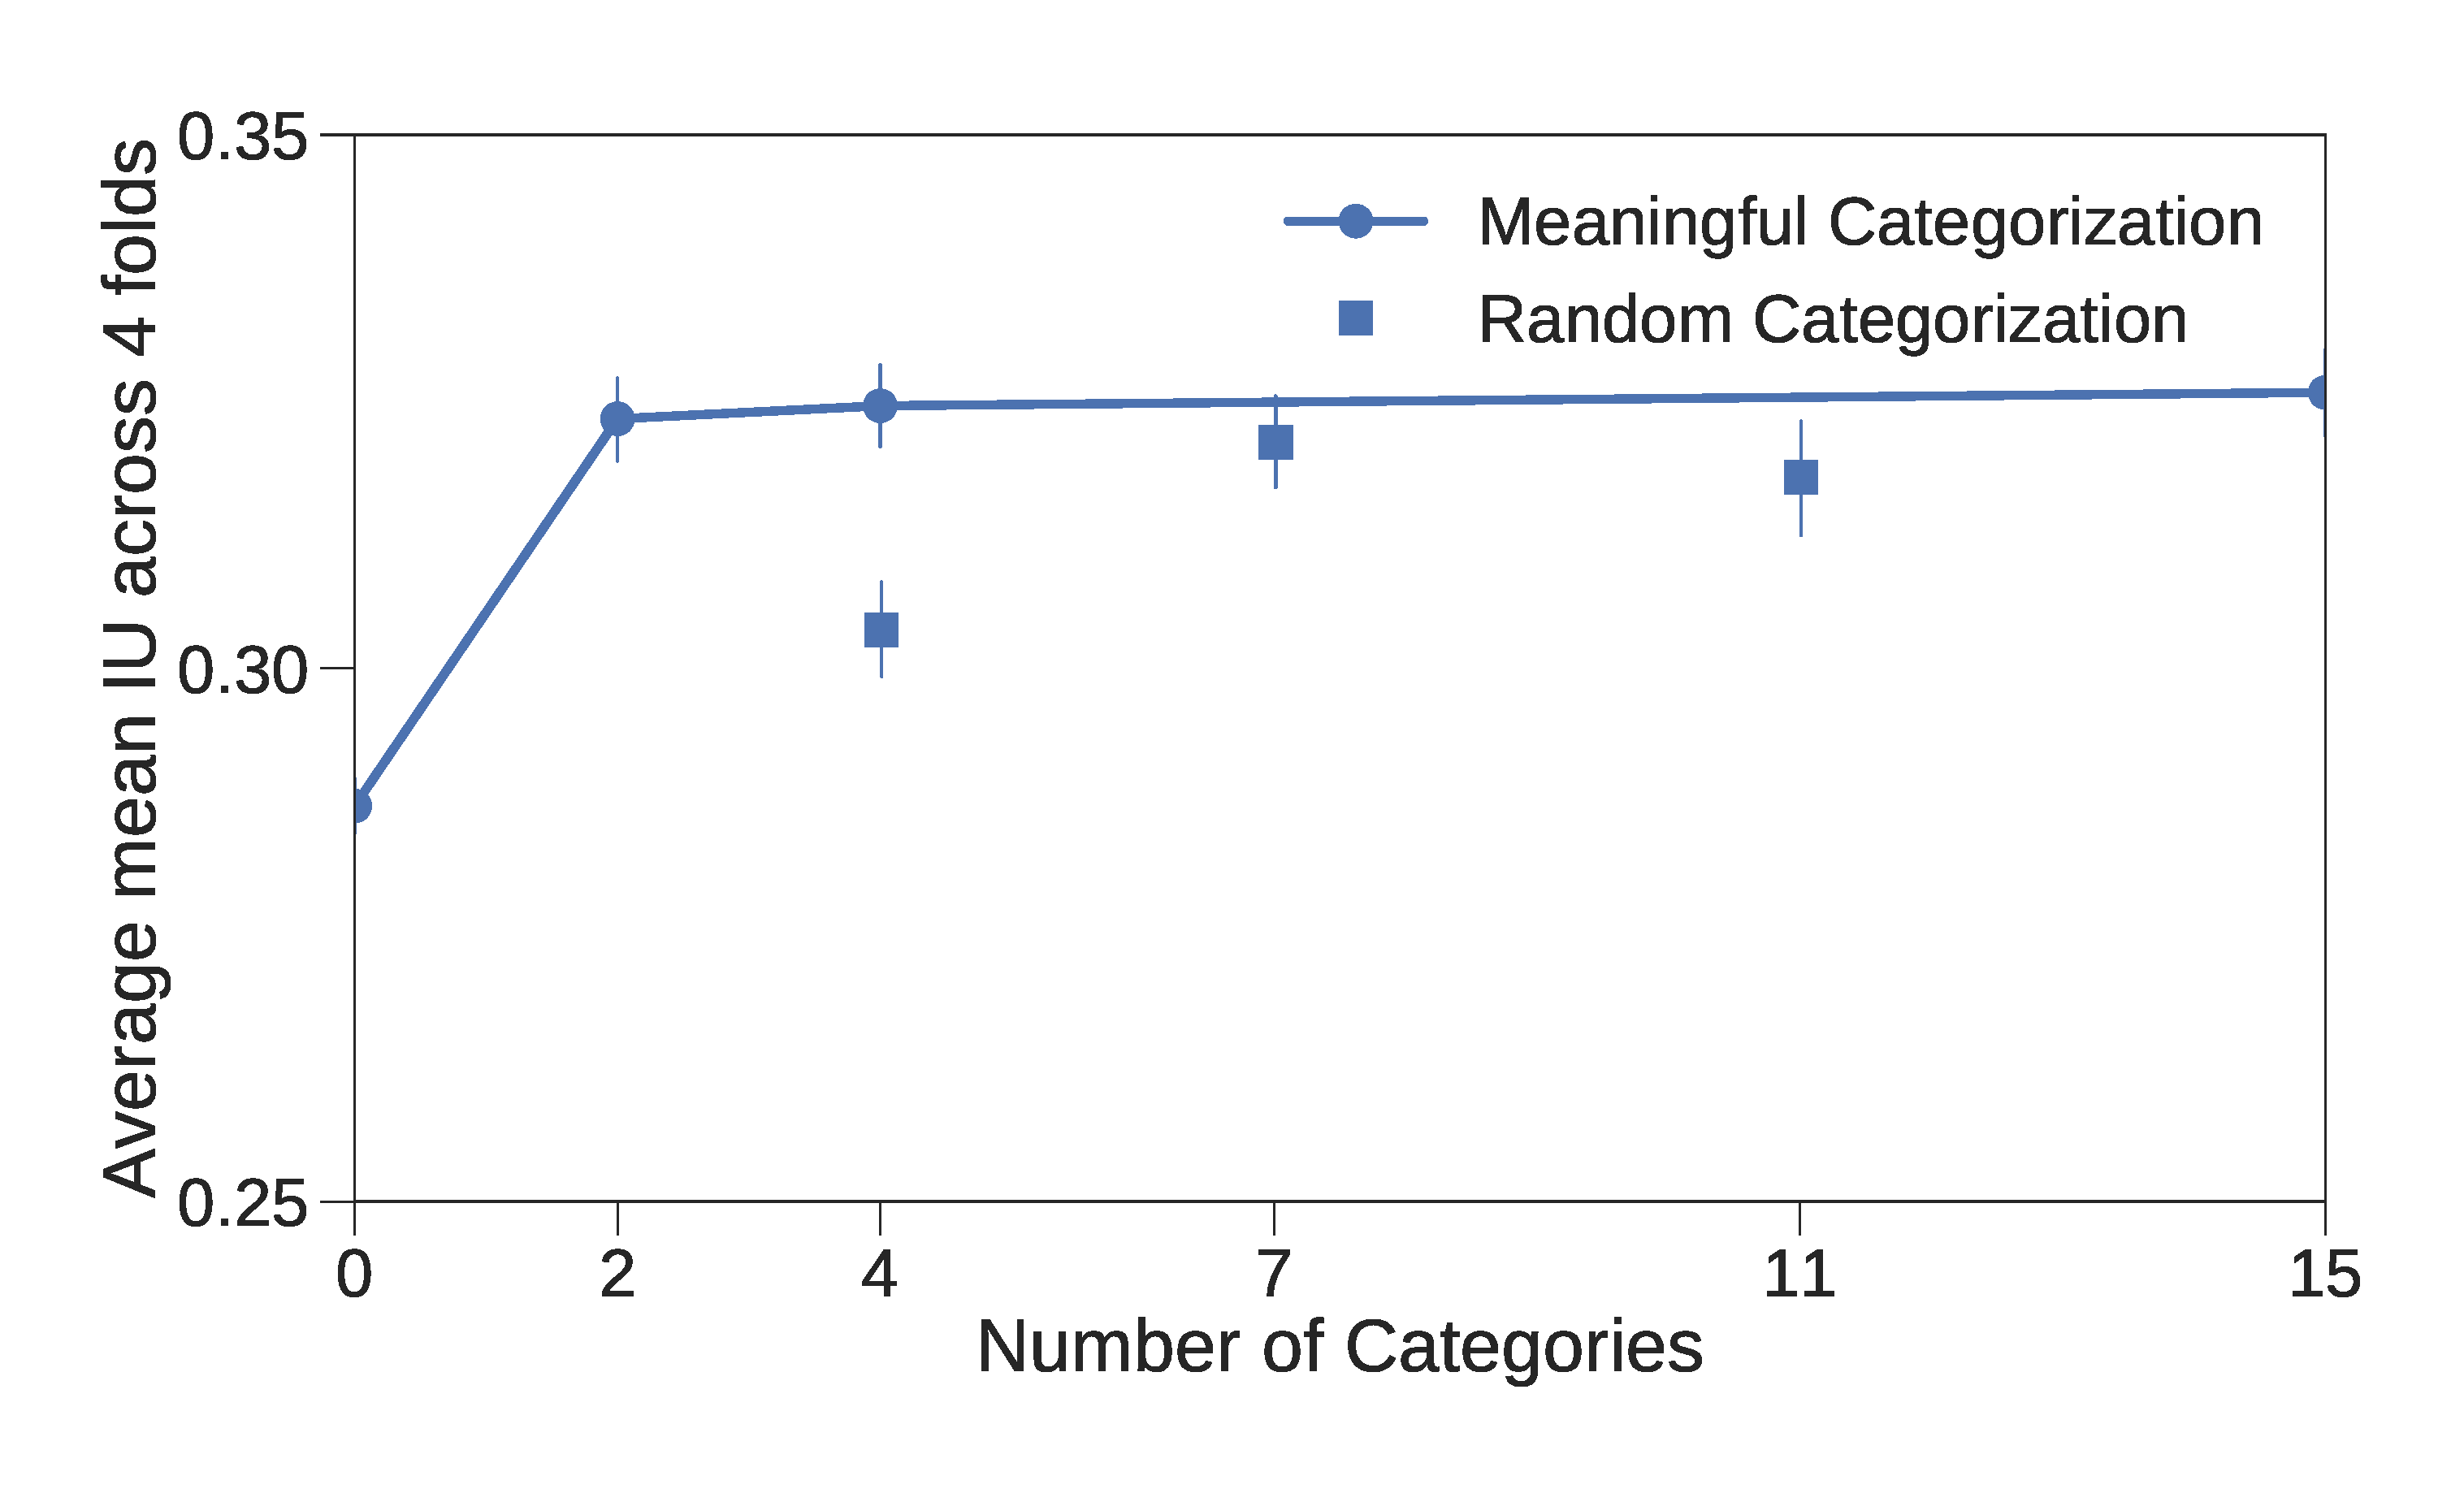
\includegraphics[width=1.\linewidth]{img/num_classes.eps}
\caption{
Test performance for the fine-tuned models pre-trained with varying categorization of pre-training classes.
Zero categorize means no pre-trained weights used and the model was random initialized.
Error bars located on lines denote the meaningful categorization, and isolated error bars denote random categorizations (RC) of the 15 classes.
The displayed mean IU/mean accuracies and standard deviations were averaged over four folds listed in Table \ref{tab:robustness}.
The line shows that binarizing and categorizing classes meaningfully had little negative effect on feature transferability.
}
\label{fig:categories}
\end{figure}


%%%%%%%%%%%%%%%%%%%%%%%%%%%%%%%%%%%%%%%%%%%%%%%%%%%%%%%%%%%%
%%%%%%%%%% PU Learning
%%%%%%%%%%%%%%%%%%%%%%%%%%%%%%%%%%%%%%%%%%%%%%%%%%%%%%%%%%%%

\subsection{Learning with only positive and unlabeled samples}
\label{subsec:pulearning}


\subsubsection{2D non-linear dataset}

To investigate the decision boundaries led by the sigmoid loss for the negative class, we trained a two-layer multilayer perceptron, with six neurons per layer, using the normal logistic loss, the class-weighted logistic loss, and the class-dependent sigmoid loss respectively and visualize the optimal decision boundaries.

\paragraph{Experimental setup}
The training data contains four hundred samples per class drawn randomly from two interleaving half circles with noises added with a minor standard deviation, as shown in Figure \ref{fig:moons}.
Half of the positive examples were assigned negative labels, resulting in a training data with reliable positive labels but noisy negative labels.
The three different losses were trained with this noisy training data, and the result decision boundaries are drawn as white regions in Figure \ref{fig:moons}.
The same multilayer perceptron classifier was also trained with true labels to present a baseline decision boundary.
The weights for positive class and negative class in the weighted logistic loss were chose to be 1 and 0.5 respectively.

% \paragraph{Weighted logistic loss vs. sigmoid loss for the negative class}
\paragraph{Results}
If trained with the sigmoid loss, the decision boundary is distant from the positive cluster with a relatively large margin as shown in Figure \ref{fig:moons}.
By contrast, the weighted logistic loss results in a decision boundary still closed to the positive examples.
For sigmoid loss, the mislabeled positive examples far away from the decision boundary do not contribute more loss than samples less distant from the decision boundary.
As a consequence, the loss derivative with respect to the model weights is larger for uncertain predictions in overall than for confident predictions, illustrated by marker sizes in Figure \ref{fig:moonsdiff}.
Therefore, training with the sigmoid loss emphasizes the positive predictions with low confidence instead of equally down-weighting all incorrect positive predictions.
The emphasization of uncertain predictions by sigmoid loss leads to a margin from the decision boundary to both positive examples and negative examples.

%%%%%%%% FIGURE MOONS

\begin{figure*}
\begin{center}
% \fbox{\rule{0pt}{2in} \rule{.9\linewidth}{0pt}}
   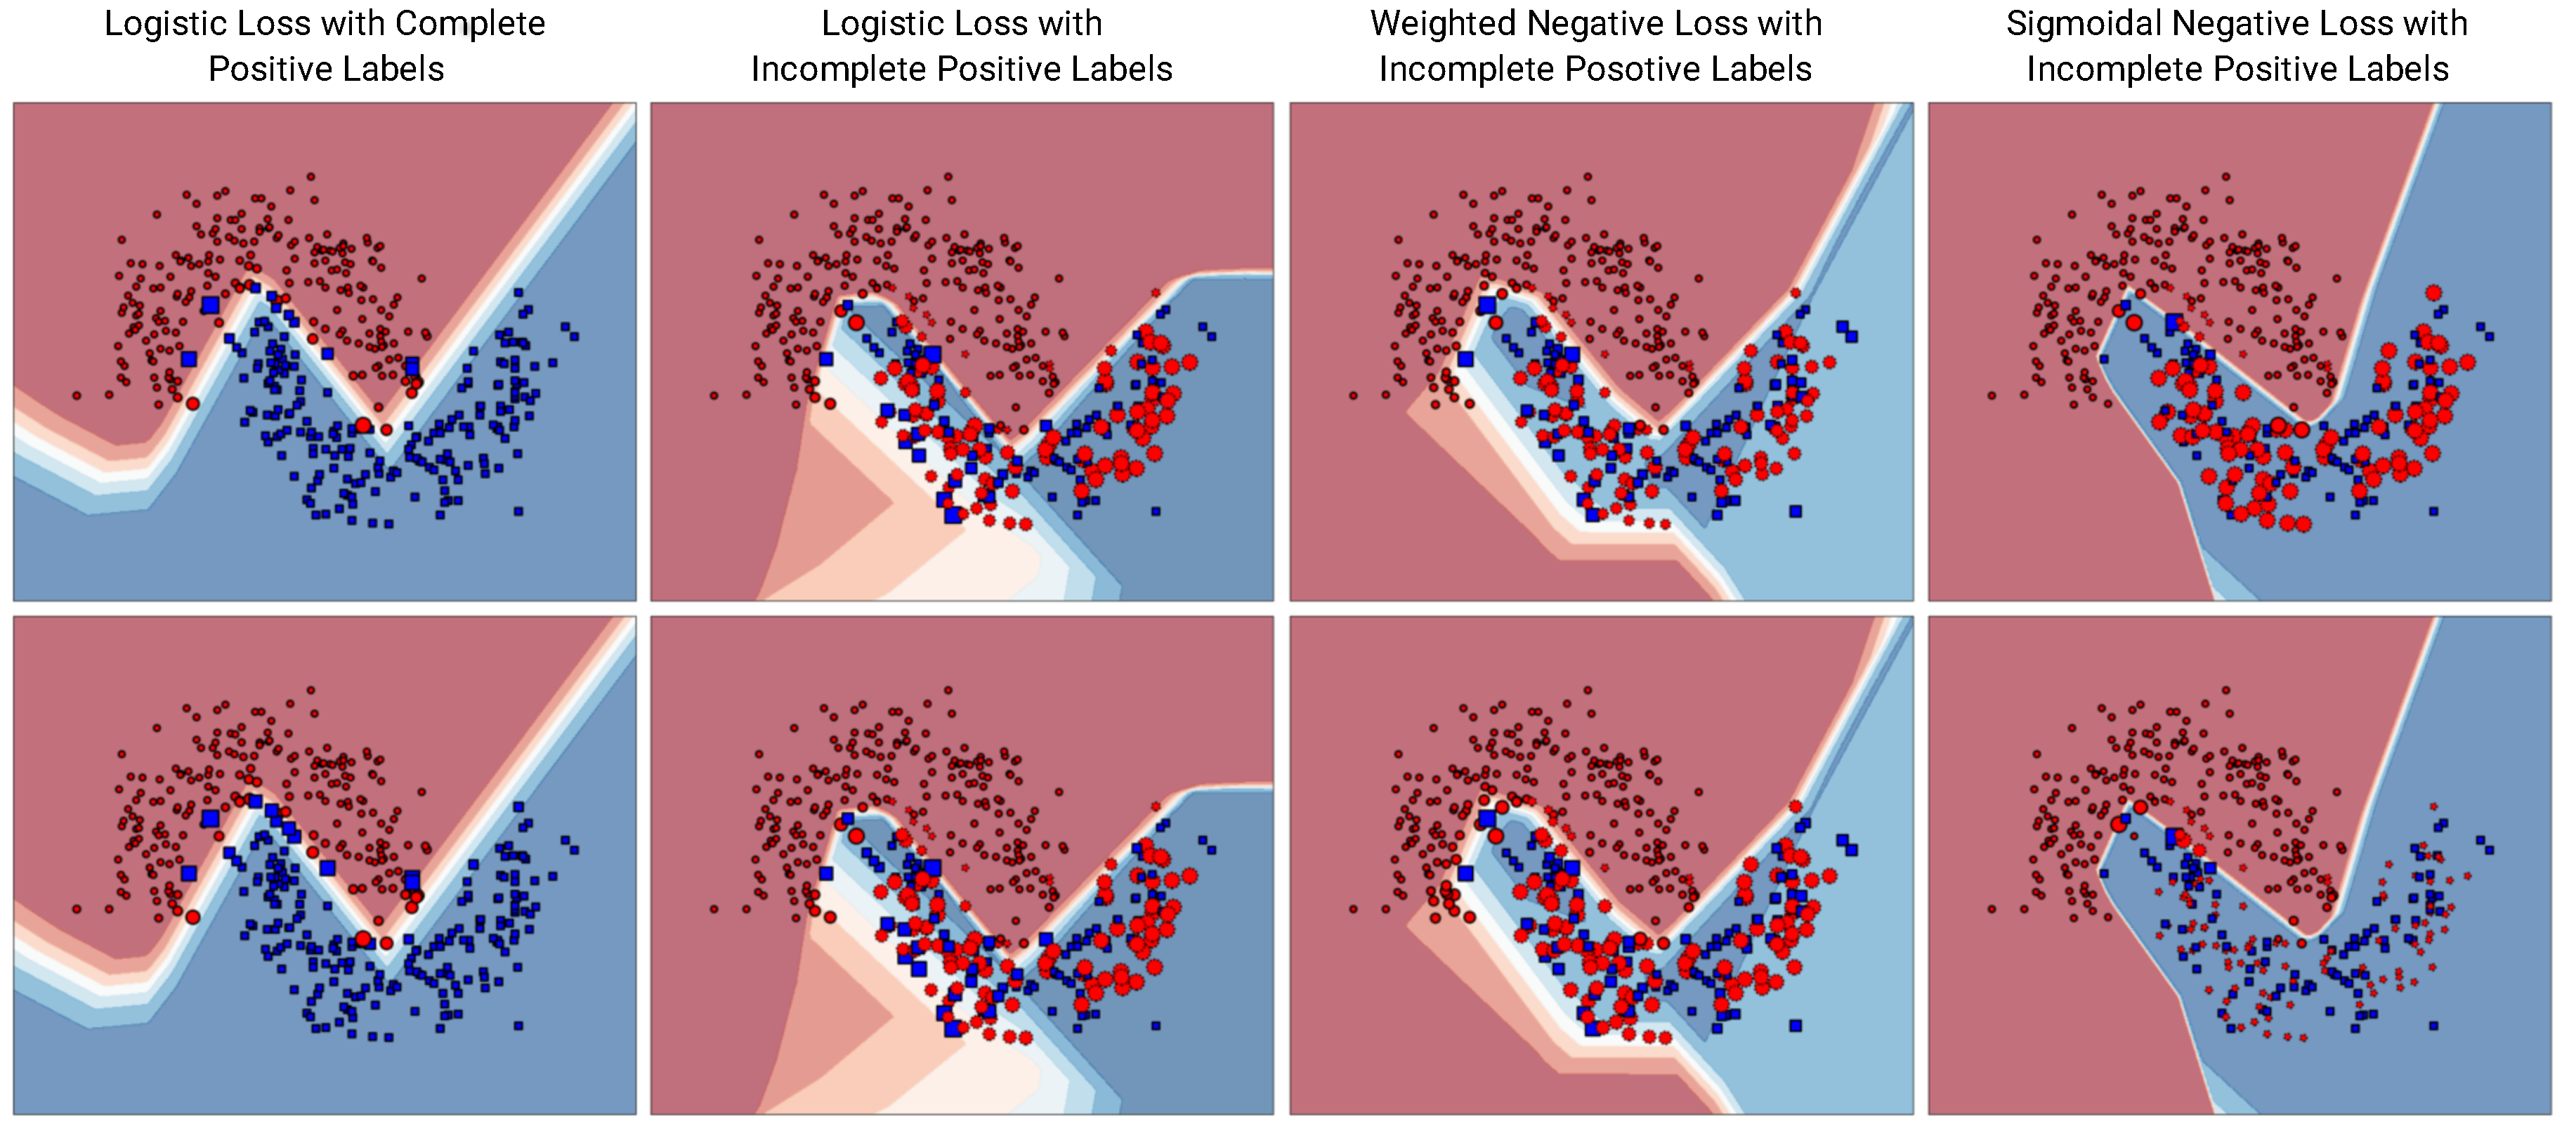
\includegraphics[width=0.95\linewidth]{img/moons.pdf}
\end{center}
   \caption{
   Decision boundaries of a 2-layer multilayer perceptron trained with different losses on a 2D moons dataset with the unlabeled positive.
  %%  The \textbf{leftmost} figures have complete positive labels, meaning the positive and negative labels are all correct, whereas, in \textbf{the other figures} only half of the positives were correctly labeled and the rest were mixed with the negative samples.
   A \textbf{red circle} indicates an example labeled as positive and a \textbf{blue square} indicates the example has a negative label.
   The \textbf{background colors} represent the classifier prediction in the corresponding area: \textbf{red} for negative class, \textbf{blue} for positive class and \textbf{white} for the class transition areas, i.e., decision boundaries.
   The \textbf{markers sizes} demonstrates the training loss normalized per-class.
   Compared to the normal logistic loss and weighted logistic loss (positive:negative=1:0.5), the decision boundary optimized with the sigmoid loss has a larger margin from the positive and negative clusters.
   (Best viewed with color)
   }
\label{fig:moons}
\end{figure*}


\begin{figure}[t]
\begin{center}
   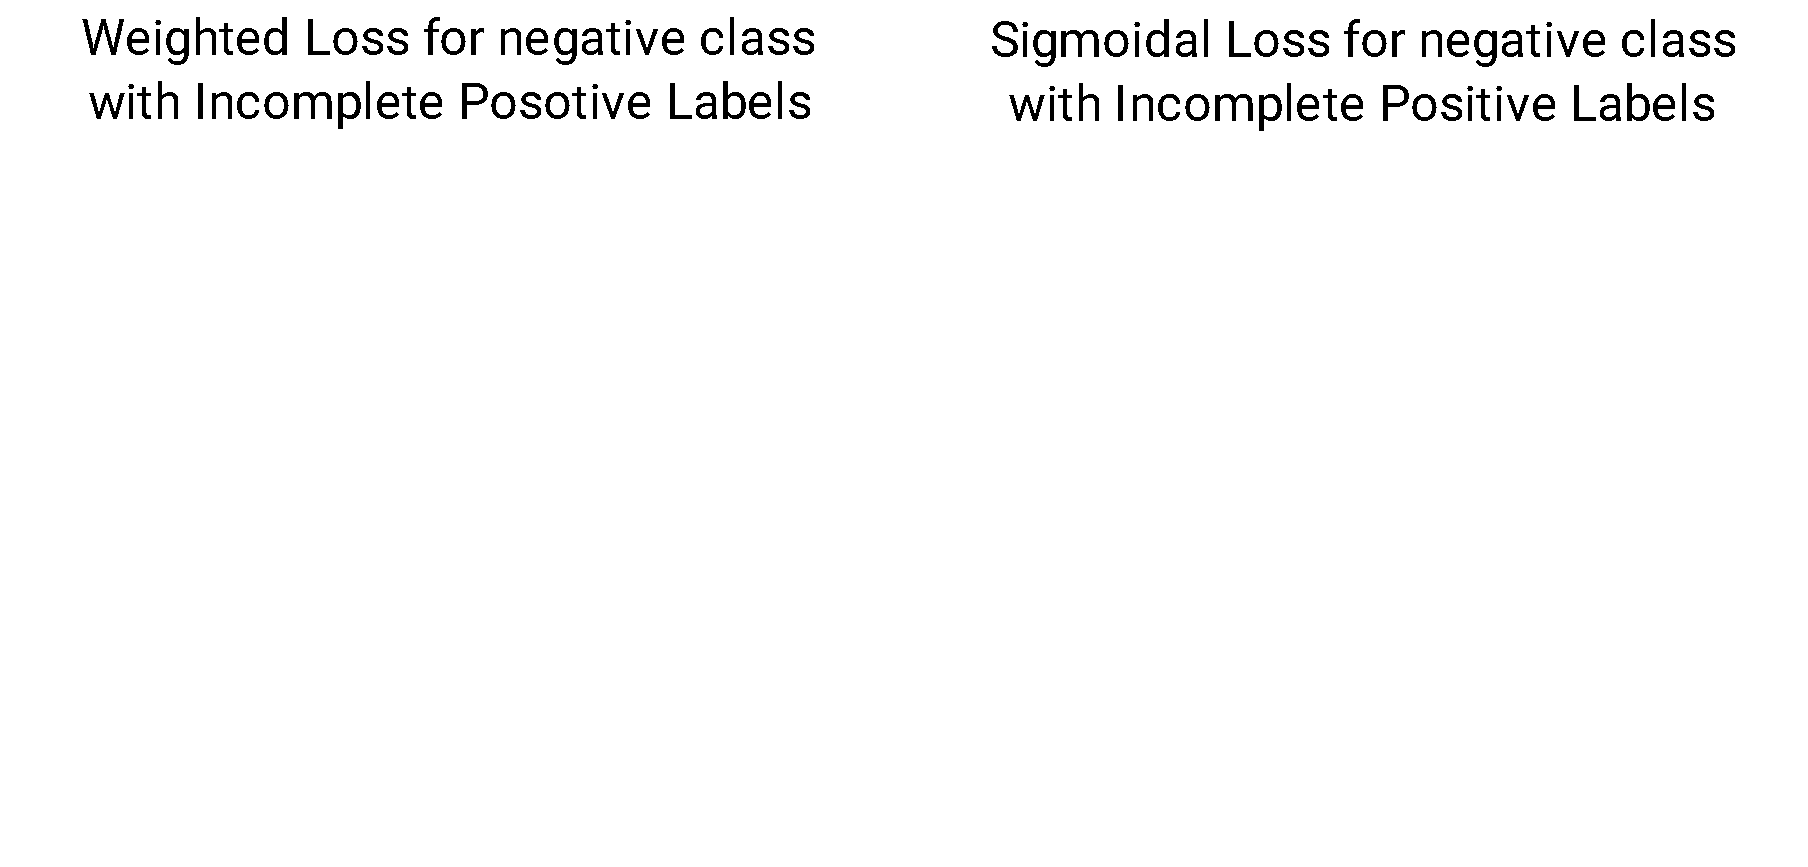
\includegraphics[width=\linewidth]{img/moons_diff}
\end{center}
   \caption{
   Derivatives w.r.t the last layer output for the two losses (normalized per class and shown as the marker size).
   The sigmoid loss has small derivatives for predictions farther from the decision boundary.
   (Best viewed with color)
   }
\label{fig:moonsdiff}
\end{figure}



\subsubsection{CIFAR dataset}

To compare the precision and recall achieved by the class-dependent softmax loss and the class-weighted cross entropy, we trained a CNN classifier to distinguish images of multiple relevant categories from non-relevant images when relevant images are partially labeled.

\paragraph{Experimental setup}
We trained an eight-layer CNN model to classify images into eleven classes: ten relevant classes from CIFAR10 and one non-relevant class for all categories from CIFAR100.
Relevant images are partially labeled, and the rest forms an unlabeled (U) set together with the non-relevant images.
An eight layer CNN model was trained with the cross-entropy loss, the class-weighted cross-entropy loss and the class-depend sigmoid loss respectively in the simulated PU learning setup, where 50\% of the positive examples were unlabeled.
The CNN model was also trained with the modified hard bootstrapping loss introduced in Section \ref{sec:pulearning} to set a benchmark for the state-of-the-art method to learn in the presence of label noises.
Model performances were evaluated on a separate test set with true labels.
The architecture of the CNN model can be found in Appendix \ref{sec:support}.
Each model was trained from scratch with Adam optimizer and base learning rate 0.0001.
Experiments were repeated three times with random split of P set, and U set and standard deviations were around 0.01 if not explicitly mentioned.
% Note that there is no category overlap between CIFAR10 dataset and CIFAR100 dataset.

%%%%%%%% TABLE CIFAR10 50%

\paragraph{Results}

Table \ref{tab:cifar} shows using the softmax loss for the non-relevant class achieves better recall than the class-weighted cross-entropy loss without lowering precision significantly.
With 50\% of the relevant examples correctly labeled and the rest assigned non-relevant labels, the normal cross-entropy loss leads to an imbalanced model with high precision but low recall, and therefore with a low f1-score.
By reweighing the loss for the non-relevant class by a factor of 0.5, the model becomes balanced for precision and recall so that the result f1-score is improved significantly.
Compared to the class-weighted cross entropy, the class-dependent softmax loss improves recall by 0.08 while reduces precision only by 0.01.
The f1-score achieved by the class-dependent softmax loss is slightly better than the class-weighted loss, though not as good as training with clean labels with either 50\% of the sample or the complete training set.
The state-of-the-art benchmark method, the hard bootstrap loss, achieves the same f1-score as the softmax loss but not as high recall.
This result is as expected because the softmax loss and the hard bootstrap loss share an idea of encouraging confident predictions.

% It is noteworthy that the weighted negative loss and hard bootstrapping loss achieved more balanced precision and recall than the sigmoid negative loss.
% That is because the two former losses were weighted by classes frequency of observed labels, around 0.67 for the negative class and 2 for positive classes, whereas the sigmoid negative loss was not.
% Reweighing the sigmoid negative loss by observed label frequencies would trade too much precision for recall (0.74 and 0.83 respectively), resulting in a worse f1-score than not reweighing losses.
% The sigmoid negative loss seems to be easier over-balancing with the same choice of class weights.
% Besides, the optimal precision and recall for sigmoid negative loss seem more unstable which may relate to the nonconvex class-dependent loss.


\begin{table}[t]
\resizebox{\columnwidth}{!}{
\centering
\begin{tabular}{ll|llll}
Annotation  & Loss & acc. & mean prec. & mean rec. & mean $F_1$ \\
\hline
R+N         & CrossEntropy   & 0.87 & 0.88 & 0.82 & 0.85 \\
50\%(R+N)   & CrossEntropy   & 0.83 & 0.84 & 0.78 & 0.80 \\
50\%R+U     & CrossEntropy   & 0.66 & 0.94 & 0.38 & 0.49 \\
\hline
50\%R+U     & ClassWeighted     & 0.78 & 0.75 & 0.75 & 0.76 \\
50\%R+U     & SoftmaxLoss      & 0.79 & 0.74 & \textbf{0.83} & \textbf{0.78} \\
50\%R+U     & BootstrapHard    & \textbf{0.80} & 0.76 & 0.81 & \textbf{0.78} \\
\end{tabular}
}
\caption{
Comparing different losses for training a 2-layer multilayer perception to classify ten relevant classes and one non-relevant class with partially labeled relevant examples and unlabeled non-relevant examples.
The trained classifiers are evaluated on a test set of true labels.
For each of the relevant classes, precision, recall, and f1-score are measured with the one-vs-all strategy and averaged.
\textbf{R+N} denotes model trained with the complete relevant labels (R set) and non-relevant labels (N set);
\textbf{50\%(R+N)} represents model trained with the half of the relevant labels and non-relevant labels respectively;
\textbf{50\%R+U} means the model is trained with half of the relevant samples, and the rest relevant samples are mixed with non-relevant samples (U set).
Weighting the non-relevant class by a factor of 0.5 improves the mean f1-score from 0.49 to 0.76.
Both the class-dependent softmax loss and the hard bootstrapping loss perform even better than simply weighing the classes, but not as good ass training with a set of labeled negative examples.
Using the softmax loss for non-relevant class achieves the highest mean recall, whereas the modified hard bootstrapping loss has a higher accuracy with 50\% positive examples unlabeled.
}
\label{tab:cifar}
\end{table}


%%%%%%%% FIGURE Varying positive annotating percetage
By varying the labeled percentage of the relevant images, Figure \ref{fig:pct_annotating} demonstrates that the class-dependent softmax loss performs slightly better than the class weighted cross-entropy when the labeled percentage of relevant images is neither too high ($>0.8$) nor too low ($<0.2$).
% When the labeled percentage of relevant images is high, the difference in loss contributions of the unlabeled relevant images for the two losses is small.
% When the percentage is low, the severe imbalance of classes introduced by unlabeled relevant images prevents the models from achieving good classification performance.

% Similarly as the result at 50\% positive examples labeled, the sigmoid loss and the hard bootstrapping loss have only little improvement compared to the weighted negative loss.
% The assumption we made for the sigmoid negative loss was that the probability of a negative example being wrong is dependent on the confidence.
% However, the synthesized mislabeled positive examples were distributed at random when we synthesized them, meaning that the probability for a negative label being wrong is independent of the underlying distribution of the inputs.
% No matter where the decision boundary is, such uniformly distributed incorrect negative labels are independent of the prediction confidence.
% Therefore, it is expected for the sigmoid negative loss and bootstrapping loss to have similar performance as the weighted negative loss.

% By varying the percentage of labeled relevant examples, the class-dependent sigmoid loss performs slightly better than the class weighted cross-entropy when the percentage of the labeled relevant images is neither too high (>0.8) nor too low (<0.2), as shown in Figure \ref{fig:pct_annotating}.
% Besides, FIgure \ref{fig:pct_annotating} demonstrates that learning with a subset of explicitly labeled non-relevant examples (RN setup) outperforms learning with the mixed unlabeled examples (RU setup) for any percentage of labeled positives and any losses being used.
% This result is expected because the explicitly labeled non-relevant examples deliver extra information about which images in the unlabeled set are non-relevant.
% Therefore, learning with positive and unlabeled examples is only relevant when it is impossible to easily construct a subset of negative examples from the unlabeled data.
% Otherwise, training with true positive and negative labels, and potentially with semi-supervised learning, would be superior to training with positive and unlabeled examples only.

\begin{figure}[t]
\centering
   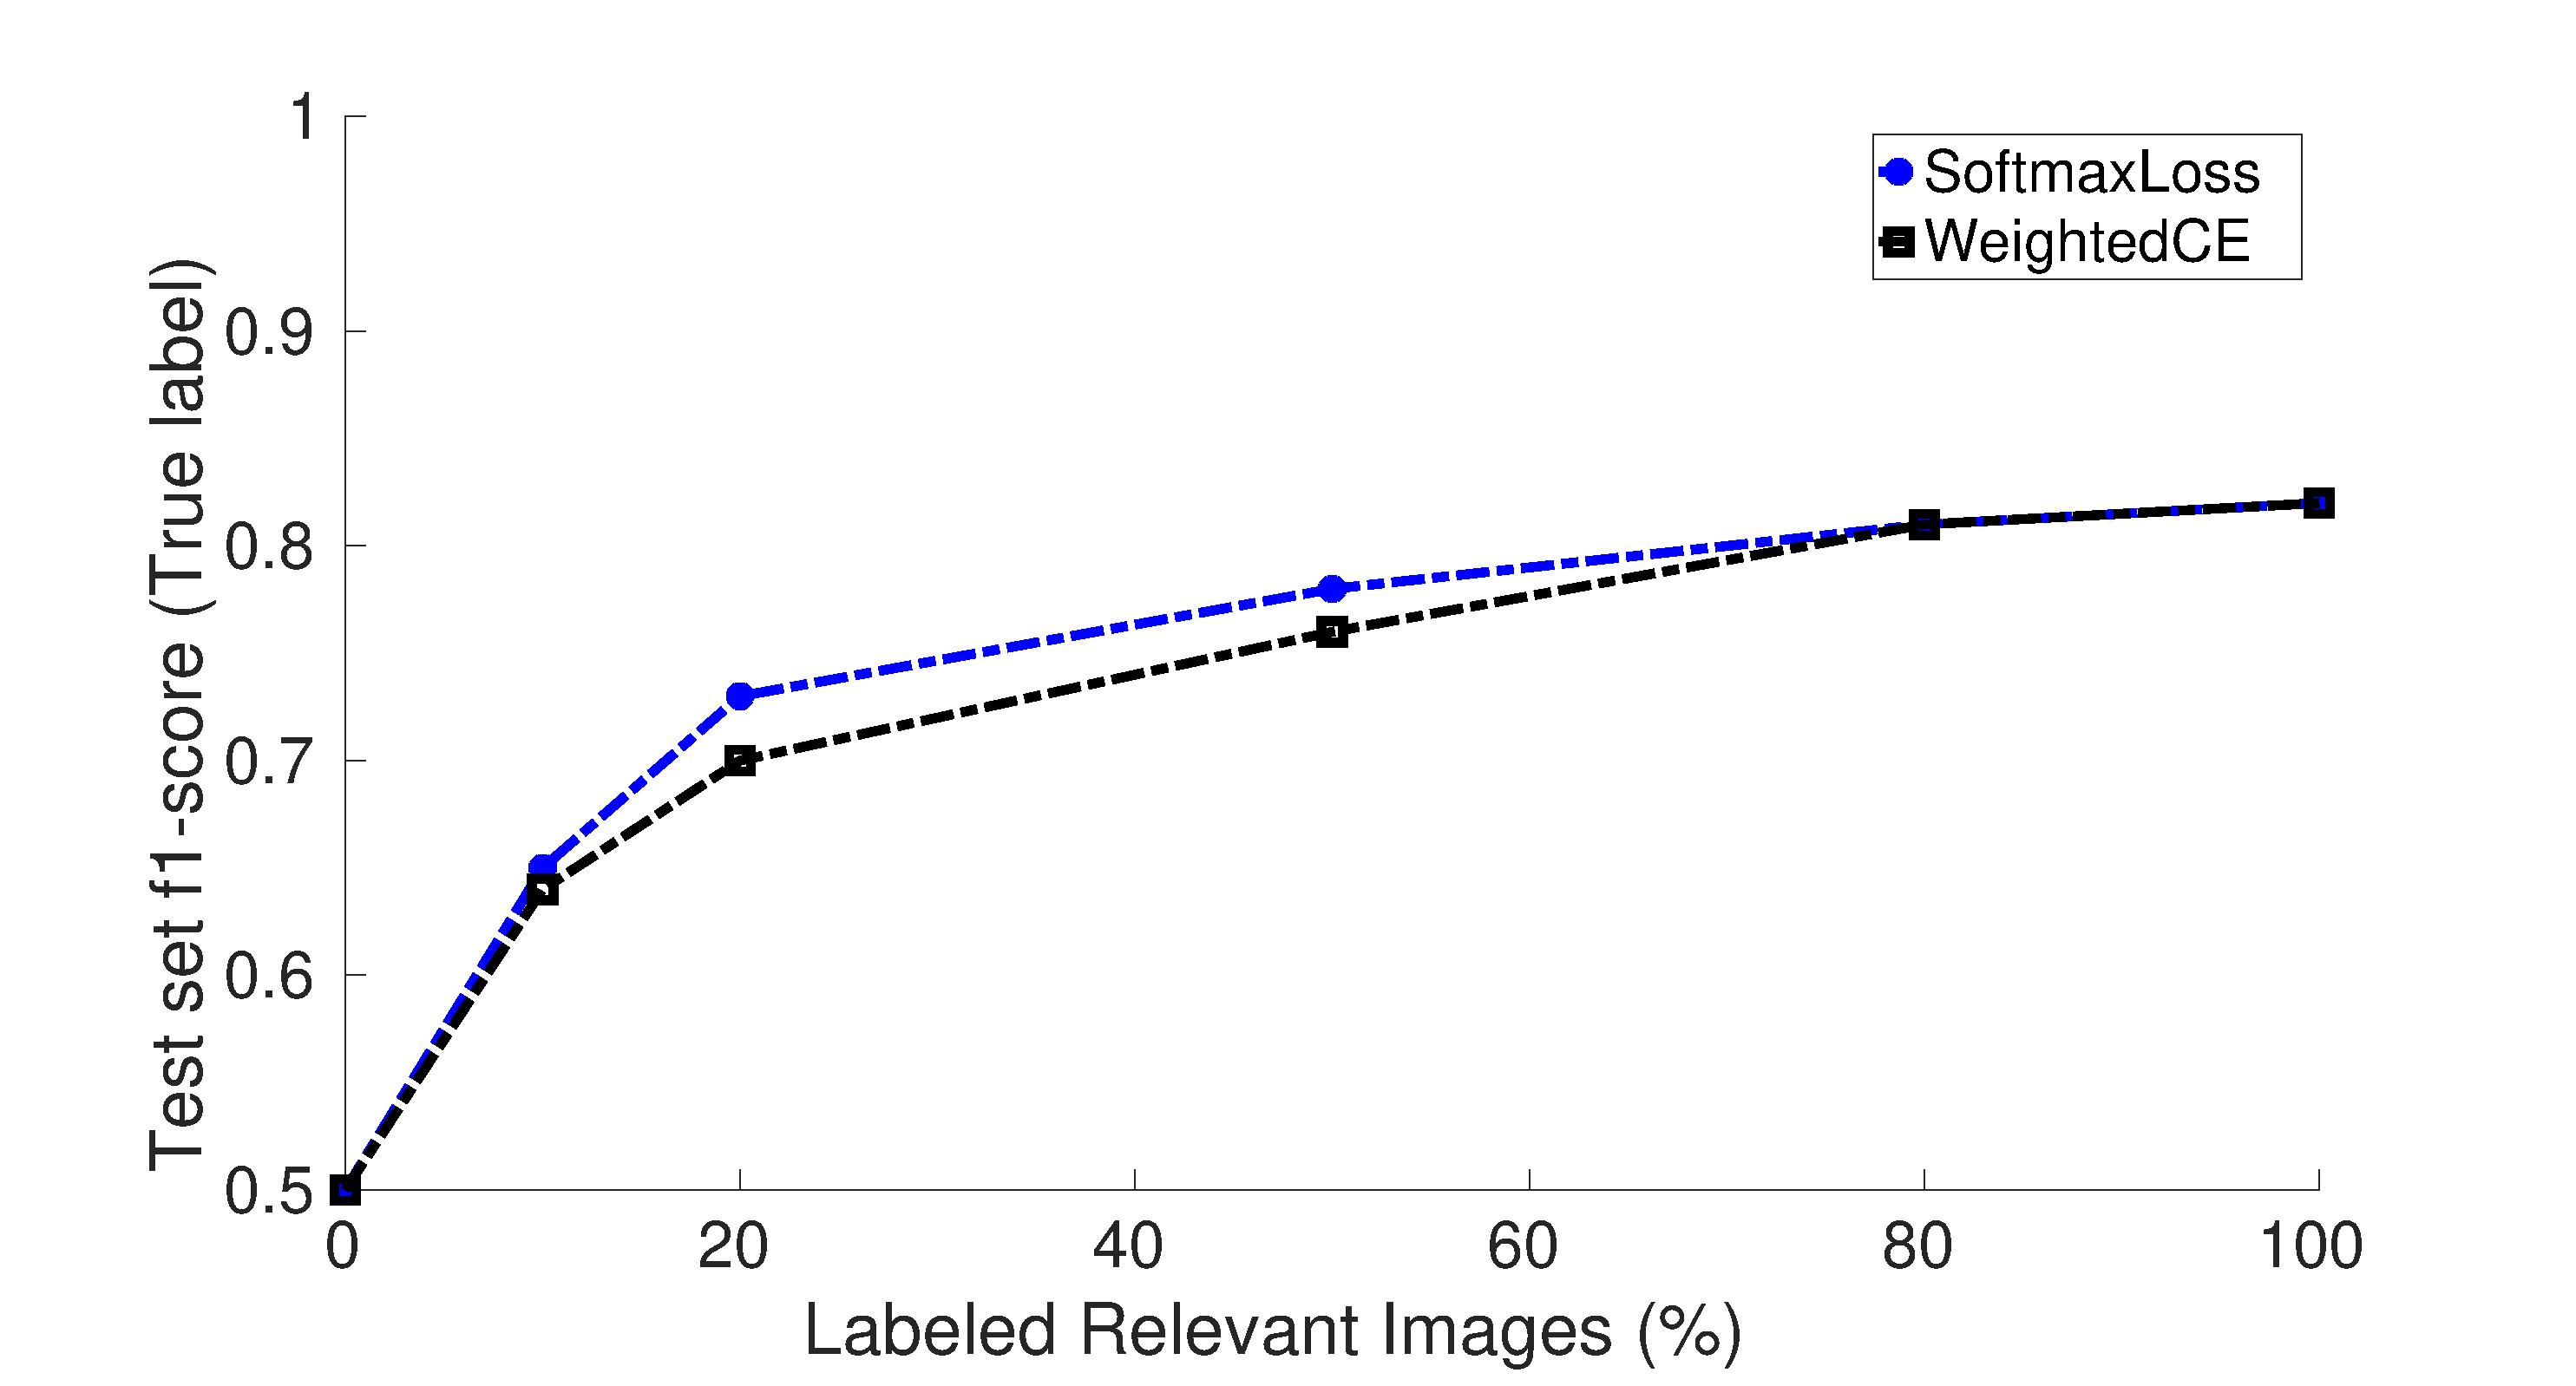
\includegraphics[width=1.05\linewidth]{img/pu_vs_pn}
\caption{
Comparing f1-score for the class-dependent softmax loss and the class-weighted cross entropy with varying percentage of relevant images labeled.
% \textbf{R+N} represents training with a percentage of reliable, relevant labels and non-relevant labels, while \textbf{R+U} stands for training with a percentage of relevant labels and all other images as unlabeled.
The class-dependent softmax loss achieves better test f1-score than the class-weighted cross entropy when 20\% and 50\% percentage of relevant images are labeled, and the others are mixed with non-relevant images.
% The class-dependent sigmoid loss achieves slightly higher f1-score than the weighted cross-entropy loss at labeled relevant  20\% and 50\% of the relevant samples are labeled.
% In general, training with explicitly labeled non-relevant examples (RN) is superior to training with an unlabeled set of mixed relevant and non-relevant examples (RU).
}
\label{fig:pct_annotating}
\end{figure}


%%%%%%%% Text Segmentation Pascal VOC2011
\subsubsection{PASCAL VOC2011 Segmentation}
To compare the class dependent sigmoid loss with the normal logistic loss, and class-weighted logistic loss for training foreground/background segmentation with incomplete segmentations, we used again the PASCAL VOC2011 dataset with extra segmentation \cite{hariharan2011semantic}.

\paragraph{Experimental setup}
We simulated inexhaustive segmentations the same way as described in Section \ref{subsec:robustness}.
The same AlexNet-FCN model was trained together with the different loss functions to predict binary segmentation, determining whether a pixel belongs to an object or not.
% Only single-object images were used for training and testing to avoid the influence of two adjacent objects joining as one object because of binary segmentation.
The same hyperparameters for optimization were used as in Section \ref{subsec:robustness}.
The trained models were evaluated with the test set of PASCAL VOC2011 segmentation dataset with binary segmentations.


\paragraph{Results}
As shown in Table \ref{tab:pusegment}, the class dependent sigmoid loss achieves the highest mean accuracy, approximately 0.07 better than training with the normal logistic loss, and 0.04 better than the class-weighted loss.
In contrast to the improvement of mean accuracy, improvement of mean IU for both the class-weigthed loss and the class-dependent logistic loss are insignificant.
The increase in the mean accuracy is caused by an increase in foreground accuracy and a decrease in background accuracy.
% The sigmoid loss increases precision for recall, similarly as observed in training the CIFAR dataset.
The decrease in background accuracy interferes the improvement mean IU since the mean IU counts for both low false positive rate and low false negative rate.


%%%%%%%% TABLE Segmentation Pascal VOC2011
\begin{table}[t]
\resizebox{\columnwidth}{!}{
\centering
\begin{tabular}{ll|llll}
Annotation  & Loss & overall acc. & mean acc. & f.w. IU & mean IU \\
\hline
% Complete            & CrossEnt.U       &  0.88 & 0.60 & 0.48 & 0.80 \\
% 50\%Unsegmented     & CrossEnt.U       &  0.83 & 0.31 & 0.27 & 0.70 \\
% 50\%Unsegmented     & WeightedU        &  0.83 & 0.34 & 0.29 & 0.70 \\
% 50\%Unsegmented     & ExponentialU     &  0.83 & 0.34 & 0.29 & 0.70 \\
Complete       & LogisticLoss       &  0.90 & 0.85 & 0.82 & 0.75 \\
50\%Unseg.     & LogisticLoss       &  0.85 & 0.68 & 0.73 & 0.60 \\
50\%Unseg.     & ClassWeighted       &  0.84 & 0.71 & 0.73 & \textbf{0.62} \\
50\%Unseg.     & SigmoidLoss      &  0.83 & \textbf{0.75} & 0.72 & \textbf{0.62} \\
\end{tabular}
}
\caption{
Training foreground/background segmentation with different losses when 50\% of the objects are unsegmented.
The performances are achieved on the test set of PASCAL VOC2011 segmentation dataset.
% A class weight of 0.7:1.75 was used to balance the sample frequency differences of the two classes.
% The negative loss was further weighted by a factor of 0.5 for the weighted negative loss.
% Mean accuracy is equivalent to the average recall over the two classes.
% Mean IU is the average intersection over union ratio (IU) over two classes and f.w. IU is the frequency weighted average of IU over the two classes.
Both the class-dependent sigmoid loss and the class-weighted logistic loss perform better than the normal logistic loss when 50\% objects unsegmented but not as good as the model trained with complete segmentations.
The class-dependent sigmoid loss has a better mean accuracy than the class-weighted logistic loss and a similar mean IU as the class-weighted logistic loss.
}
\label{tab:pusegment}
\end{table}


%%%%%%%% Figure Segmentation Pascal VOC2011
Selective predictions made by the models trained with the sigmoid negative loss and the cross entropy loss were presented in Figure \ref{fig:pusegment}.
For the two example images shown, the model trained with the cross entropy loss failed to segment objects from images whereas sigmoid negative loss predicted segmentations on the position of the objects.
The coarse outlines were mainly due to the limited compacity of the FCN-AlexNet model.
The third column shows predictions given by model trained with complete training segmentation, and it did not produce more accurate outlines.
There is no example observed correctly segmented by the model with the class-weighted logistic loss but not by the model with the class-dependent sigmoid loss.

\begin{figure}
\centering
  \begin{minipage}{\columnwidth}\footnotesize
  \centering
  \subsubfloat{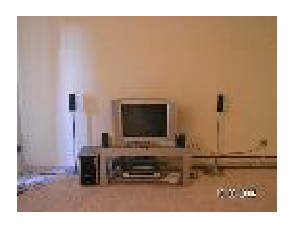
\includegraphics[width=0.19\columnwidth]{img/2007_002132}}{Raw}
  \subsubfloat{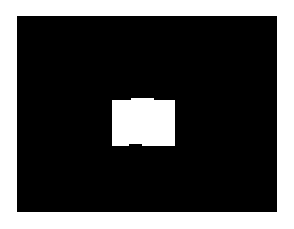
\includegraphics[width=0.19\columnwidth]{img/2007_002132_label}}{Label}
  \subsubfloat{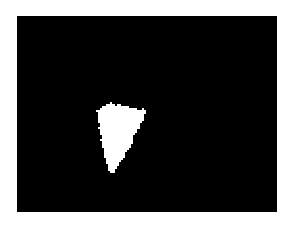
\includegraphics[width=0.19\columnwidth]{img/2007_002132_up_pred}}{Complete}
  \subsubfloat{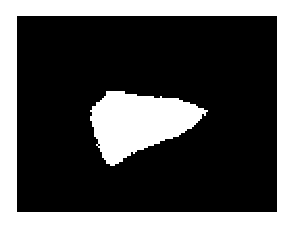
\includegraphics[width=0.19\columnwidth]{img/2007_002132_exp_pred}}{SigmoidLoss}
  \subsubfloat{
\includegraphics[width=0.19\columnwidth]{img/2007_002132_low_pred}}{ClassWeight.}
  \subsubfloat{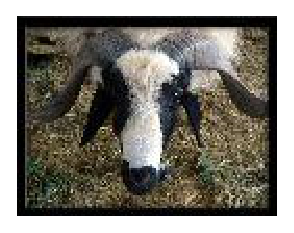
\includegraphics[width=0.19\columnwidth]{img/2007_002618}}{Raw}%
  \subsubfloat{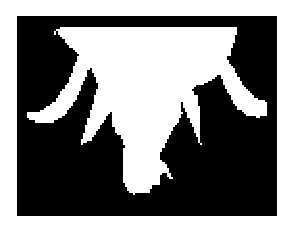
\includegraphics[width=0.19\columnwidth]{img/2007_002618_label}}{Label}
  \subsubfloat{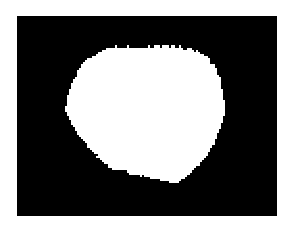
\includegraphics[width=0.19\columnwidth]{img/2007_002618_up_pred}}{Complete}
  \subsubfloat{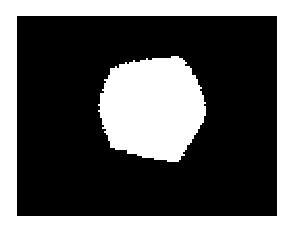
\includegraphics[width=0.19\columnwidth]{img/2007_002618_exp_pred}}{SigmoidLoss}
  \subsubfloat{
\includegraphics[width=0.19\columnwidth]{img/2007_002618_low_pred}}{ClassWeight.}
  \end{minipage}
\caption{
Example predictions made by models trained with the logistic loss and the class-dependent sigmoid loss.
This figure presented two selective images for which the model trained with the logistic loss failed to segment objects, whereas the model trained with the class-dependent sigmoid negative loss succeed.
}
\label{fig:pusegment}
\end{figure}
